%% =====================================================================
%% 武汉大学数学与统计学院 本科毕业论文（设计） —— 主文件
%% 编译：latexmk -xelatex main.tex （自动完成 xelatex → bibtex → xelatex）
%% 手动：xelatex main.tex → bibtex main → xelatex main.tex → xelatex main.tex
%% =====================================================================
\documentclass{whu-math-thesis}

%% 参考文献：GB/T 7714（natbib + gbt7714 + BibTeX）
%% 采用 BibTeX 后端，不依赖 biber，本地与 Overleaf 均可编译
\usepackage{natbib}
\usepackage[sort&compress]{gbt7714}
\bibliographystyle{gbt7714-numerical}
\usepackage[unicode,hidelinks]{hyperref}

%% ------------------------ 填写区：只改这里 ------------------------
\ctitle{一类椭圆型方程有限元方法的误差估计}
\cschool{数学与统计学院}
\cmajor{数学与应用数学}       % 亦可用：信息与计算科学 / 统计学 / 数学基地班等
\cauthor{张三}
\cnumber{2022300000000}
\cadvisor{李四\quad 教授}
\cdate{二〇二七年五月}
%% ------------------------------------------------------------------

\begin{document}

%% 封面、声明（无页码）
\maketitlepage
\makestatement

%% 前言部分（罗马页码）
\pagenumbering{Roman}
% 中英文摘要（以下为示例内容，撰写论文时请替换）
\phantomsection
\addcontentsline{toc}{chapter}{摘\hspace{1em}要}
\begin{cnabstract}{椭圆型方程；有限元方法；误差估计；数值实验}
本文以一类二阶椭圆型边值问题为研究对象，讨论其弱形式、有限元离散以及相应的先验误差估计。
首先在 Sobolev 空间框架下给出变分问题，并利用 Lax--Milgram 定理证明弱解的存在唯一性；
其次构造协调有限元空间，借助 Céa 引理与插值误差估计得到能量范数和 $L^2$ 范数下的收敛阶；
最后通过数值实验验证理论结果，考察不同网格尺度下误差的收敛行为。
文中给出的定理、公式、表格与图形均为模板示例，用于展示数学论文的写作与排版方式。
\end{cnabstract}

\phantomsection
\addcontentsline{toc}{chapter}{ABSTRACT}
\begin{enabstract}{elliptic equation; finite element method; error estimate; numerical experiment}
This thesis studies a class of second-order elliptic boundary value problems, including their
weak formulation, finite element discretization and a priori error estimates. Within the
framework of Sobolev spaces, the existence and uniqueness of the weak solution are established
by the Lax--Milgram theorem. A conforming finite element space is then constructed, and
convergence rates in the energy norm and in the $L^2$ norm are derived via Céa's lemma and
interpolation estimates. Numerical experiments are presented to illustrate the theoretical
results. All theorems, tables and figures in this template are illustrative examples.
\end{enabstract}
     % 中文摘要、英文摘要
\makecontents                % 目录
% 主要符号表（数学论文常用；按自己的记号增删）
\chapter*{主要符号表}
\addcontentsline{toc}{chapter}{主要符号表}

\begin{center}
\begin{tabular}{cl}
\toprule
符号 & 含义 \\
\midrule
$\Omega$               & $\R^n$ 中的有界开区域，边界为 $\partial\Omega$ \\
$L^2(\Omega)$          & $\Omega$ 上平方可积函数构成的 Hilbert 空间 \\
$H^1(\Omega)$          & 一阶弱导数属于 $L^2(\Omega)$ 的 Sobolev 空间 \\
$H_0^1(\Omega)$        & $H^1(\Omega)$ 中在 $\partial\Omega$ 上迹为零的子空间 \\
$\norm{\cdot}$         & 相应空间上的范数 \\
$\inner{\cdot}{\cdot}$ & 内积或 $H'$ 与 $H$ 之间的对偶配对 \\
$a(\cdot,\cdot)$       & 双线性型 \\
$\mathcal{T}_h$        & 网格尺寸为 $h$ 的剖分 \\
$V_h$                  & 有限元空间，$V_h\subset H_0^1(\Omega)$ \\
$u,\,u_h$              & 精确解与有限元数值解 \\
\bottomrule
\end{tabular}
\end{center}

\noindent 未被列出的局部记号将在首次出现时另行说明。
      % 主要符号表

%% 正文部分（阿拉伯页码）
\startmainmatter
% 第 1 章 绪论（以下为示例内容，撰写论文时请替换）
\chapter{绪论}

\section{研究背景与意义}

二阶椭圆型方程是偏微分方程理论中最基本的模型之一，广泛应用于稳态热传导、弹性力学与多孔介质渗流等问题。
由于解析解一般难以求得，数值方法成为研究这类方程的主要手段。有限元方法基于变分原理，
能够自然地处理复杂区域与边界条件，并具有较为完善的误差分析理论\cite{ciarlet1978,brenner2008}。

\section{国内外研究现状}

有限元方法的数学理论在二十世纪中后期逐步建立：变分形式与弱解理论可参见 \cite{evans2010,lax1954}，
Sobolev 空间工具可参见 \cite{adams2003}，而离散格式的一般分析框架可参见 \cite{strang1973}。
在此基础上，协调有限元、非协调有限元及自适应方法相继发展，误差估计与收敛性分析已成为标准工具。

\section{本文的主要工作}

本文围绕模型问题
\begin{equation}\label{eq:model}
-\Delta u + u = f \quad \text{in } \Omega, \qquad u = 0 \quad \text{on } \partial\Omega,
\end{equation}
完成以下工作：

\begin{enumerate}[label=(\arabic*)]
  \item 给出问题 \eqref{eq:model} 的弱形式，并证明弱解的存在唯一性；
  \item 构造分片线性协调有限元空间，推导能量范数与 $L^2$ 范数下的先验误差估计；
  \item 设计数值实验，验证收敛阶并讨论网格尺度对计算精度的影响。
\end{enumerate}

\section{论文结构安排}

第 2 章整理所需的函数空间与基本不等式；第 3 章给出主要定理及其证明；
第 4 章展示算法实现与数值结果；第 5 章总结全文并展望未来工作。
     % 绪论
% 第 2 章 预备知识（以下为示例内容，撰写论文时请替换）
\chapter{预备知识}

\section{记号与函数空间}

设 $\Omega\subset\R^n$ 为有界 Lipschitz 区域。记 $L^2(\Omega)$ 上的内积与范数为
\begin{equation}\label{eq:l2}
\inner{u}{v}_{L^2(\Omega)}=\int_\Omega u v \dd x, \qquad
\norm{u}_{L^2(\Omega)}=\sqrt{\inner{u}{u}_{L^2(\Omega)}}.
\end{equation}

\begin{definition}[Sobolev 空间 $H^1(\Omega)$]
$H^1(\Omega)=\bigl\{u\in L^2(\Omega):\ \partial_{x_i}u\in L^2(\Omega),\ i=1,\dots,n\bigr\}$，
其中导数在弱意义下理解；$H_0^1(\Omega)$ 表示 $C_c^\infty(\Omega)$ 在 $H^1$ 范数下的闭包。
\end{definition}

\section{基本不等式与引理}

\begin{lemma}[Cauchy--Schwarz 不等式]\label{lem:cs}
对任意 $u,v\in L^2(\Omega)$，有
\begin{equation}\label{eq:cs}
\abs{\int_\Omega u v \dd x}\le \norm{u}_{L^2(\Omega)}\norm{v}_{L^2(\Omega)}.
\end{equation}
\end{lemma}

\begin{proof}
对任意 $\lambda\in\R$，由 $\int_\Omega (u-\lambda v)^2\dd x\ge 0$ 展开得
$\norm{u}^2-2\lambda\inner{u}{v}+\lambda^2\norm{v}^2\ge 0$。
取 $\lambda=\inner{u}{v}/\norm{v}^2$（$\norm{v}=0$ 时结论显然），即得 \eqref{eq:cs}。
\end{proof}

\begin{remark}
引理 \ref{lem:cs} 在 Hilbert 空间 $H$ 上同样成立，只需把 $L^2$ 内积换成 $H$ 的内积；
本文后续均在 $H=H_0^1(\Omega)$ 上使用这一形式。
\end{remark}

\section{弱形式}

对式 \eqref{eq:model} 两边乘以测试函数 $v\in H_0^1(\Omega)$ 并在 $\Omega$ 上分部积分，得到
\begin{equation}\label{eq:weak-form}
a(u,v)\coloneqq \int_\Omega \bigl(\nabla u\cdot\nabla v + uv\bigr)\dd x
= \int_\Omega f v \dd x, \qquad \forall v\in H_0^1(\Omega).
\end{equation}
由式 \eqref{eq:cs} 可知 $a(\cdot,\cdot)$ 有界；再由 Poincaré 不等式可得其强制性。
     % 预备知识
% 第 3 章 主要结果与证明（以下为示例内容，撰写论文时请替换）
\chapter{主要结果与证明}

\section{弱解的存在唯一性}

\begin{theorem}[Lax--Milgram 定理]\label{thm:lm}
设 $H$ 为实 Hilbert 空间，$a(\cdot,\cdot)$ 为 $H\times H$ 上的双线性型，
且存在常数 $M,\alpha>0$ 使得对任意 $u,v\in H$ 有
$\abs{a(u,v)}\le M\norm{u}_H\norm{v}_H$ 与 $a(u,u)\ge \alpha\norm{u}_H^2$。
则对任意 $f\in H'$，存在唯一的 $u\in H$ 满足
\begin{equation}\label{eq:lm}
a(u,v)=\langle f,v\rangle, \qquad \forall v\in H,
\end{equation}
并且 $\norm{u}_H\le \alpha^{-1}\norm{f}_{H'}$。
\end{theorem}

\begin{proof}
对每个固定的 $u\in H$，映射 $v\mapsto a(u,v)$ 是 $H$ 上的有界线性泛函，
由 Riesz 表示定理存在唯一 $Au\in H$ 使得 $a(u,v)=\inner{Au}{v}_H$。
强制性给出 $\alpha\norm{u}_H^2\le a(u,u)=\inner{Au}{u}_H\le\norm{Au}_H\norm{u}_H$，
从而 $A$ 单射且值域闭；再由 $A$ 的伴随算子同理可证值域稠密，故 $A$ 为双射，
式 \eqref{eq:lm} 存在唯一解。估计式由 $\alpha\norm{u}_H^2\le\langle f,u\rangle\le\norm{f}_{H'}\norm{u}_H$ 得到。
\end{proof}

\begin{corollary}\label{cor:exist}
变分问题 \eqref{eq:weak-form} 存在唯一弱解 $u\in H_0^1(\Omega)$，且
$\norm{u}_{H^1(\Omega)}\le C\norm{f}_{L^2(\Omega)}$，其中 $C$ 仅依赖于 $\Omega$。
\end{corollary}

\section{有限元离散与误差估计}

设 $\mathcal{T}_h$ 为 $\Omega$ 的拟一致剖分，$V_h\subset H_0^1(\Omega)$ 为分片线性有限元空间。
离散问题为：求 $u_h\in V_h$ 使得
\begin{equation}\label{eq:discrete}
a(u_h,v_h)=\int_\Omega f v_h \dd x,\qquad \forall v_h\in V_h.
\end{equation}

\begin{proposition}[Céa 引理]\label{prop:cea}
设 $u$ 与 $u_h$ 分别为 \eqref{eq:weak-form} 与 \eqref{eq:discrete} 的解，则
\begin{equation}\label{eq:cea}
\norm{u-u_h}_{H^1(\Omega)}\le \frac{M}{\alpha}\inf_{v_h\in V_h}\norm{u-v_h}_{H^1(\Omega)}.
\end{equation}
\end{proposition}

\begin{proof}
由 Galerkin 正交性 $a(u-u_h,v_h)=0$ 及强制性、有界性，
取 $v_h=u_h-w_h$（$w_h\in V_h$ 任意）即得 \eqref{eq:cea}。
\end{proof}

\begin{example}
若 $u\in H^2(\Omega)$，由插值估计 $\inf_{v_h\in V_h}\norm{u-v_h}_{H^1}\le Ch\abs{u}_{H^2}$
及式 \eqref{eq:cea} 可得能量范数下的一阶收敛；结合 Aubin--Nitsche 技巧可得
$\norm{u-u_h}_{L^2(\Omega)}=O(h^2)$。第 4 章的数值实验将验证这一收敛阶。
\end{example}

\begin{remark}
上述结论对更一般的 coercive 双线性型同样成立；若采用非协调元或间断有限元方法，
则需相应修改证明，可参见 \cite{brenner2008,ciarlet1978}。
\end{remark}
     % 主要结果与证明
% 第 4 章 数值实验（以下为示例内容、示例数据，撰写论文时请替换）
\chapter{数值实验}

\section{算法实现}

取 $\Omega=(0,1)^2$，真解 $u(x,y)=\sin(\pi x)\sin(\pi y)$，右端项由式 \eqref{eq:model} 确定。
在均匀三角形网格 $\mathcal{T}_h$ 上采用分片线性协调有限元，求解流程见算法 \ref{alg:fem}。

\begin{algorithm}[htbp]
\caption{有限元求解流程（示例）}\label{alg:fem}
\KwIn{网格 $\mathcal{T}_h$、右端项 $f$}
\KwOut{数值解 $u_h$ 与误差 $\norm{u-u_h}_{L^2(\Omega)}$}
组装刚度矩阵 $A$ 与载荷向量 $\vect{b}$\;
施加齐次 Dirichlet 边界条件\;
求解线性方程组 $A\vect{u}=\vect{b}$\;
由 $\vect{u}$ 重构 $u_h$，并按式 \eqref{eq:l2} 计算误差\;
\end{algorithm}

\section{误差与收敛阶}

表 \ref{tab:error} 列出了不同网格尺度下的自由度、$L^2$ 误差与收敛阶。
表中数值仅用于演示三线表排版，并非真实计算结果。

\begin{table}[htbp]
\centering
\caption{不同网格尺度下的误差与收敛阶（示例数据）}\label{tab:error}
\begin{tabular}{cccc}
\toprule
$h$ & 自由度 & $\norm{u-u_h}_{L^2(\Omega)}$ & 收敛阶 \\
\midrule
$1/8$   & $81$   & $3.12\times10^{-2}$ & --   \\
$1/16$  & $289$  & $7.94\times10^{-3}$ & $1.97$ \\
$1/32$  & $1089$ & $2.01\times10^{-3}$ & $1.98$ \\
$1/64$  & $4225$ & $5.06\times10^{-4}$ & $1.99$ \\
\bottomrule
\end{tabular}
\end{table}

图 \ref{fig:conv} 在双对数坐标下给出了误差随 $h$ 的变化，
虚线为参考斜率 $O(h^2)$，与第 3 章例中的理论预测一致。

\begin{figure}[htbp]
\centering
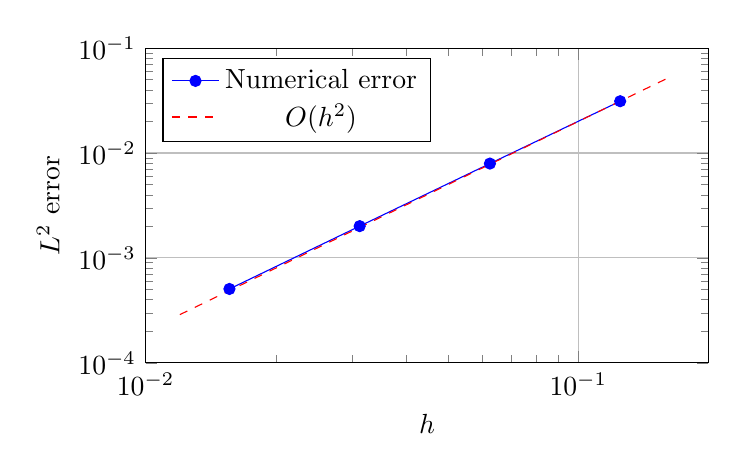
\begin{tikzpicture}
\begin{loglogaxis}[
  width=0.72\textwidth, height=0.46\textwidth,
  xlabel={$h$}, ylabel={$L^2$ error},
  grid=major, legend pos=north west,
  xmin=0.01, xmax=0.2, ymin=1e-4, ymax=1e-1]
\addplot[mark=*,blue] coordinates {
  (0.125,0.0312) (0.0625,0.00794) (0.03125,0.00201) (0.015625,0.000506)};
\addplot[dashed,red,domain=0.012:0.16] {2*x^2};
\legend{Numerical error, $O(h^2)$}
\end{loglogaxis}
\end{tikzpicture}
\caption{$L^2$ 误差的收敛曲线（示例）}\label{fig:conv}
\end{figure}

\section{结果分析}

由表 \ref{tab:error} 可见，随着 $h$ 减半，$L^2$ 误差约降至原来的 $1/4$，
收敛阶稳定在 $2$ 附近，与命题 \ref{prop:cea} 结合插值估计得到的结论相符。
误差主要来源于空间离散；若改用更高次单元或自适应网格，可进一步提高计算效率。
     % 数值实验
% 第 5 章 总结与展望（以下为示例内容，撰写论文时请替换）
\chapter{总结与展望}

\section{全文总结}

本文以模型问题 \eqref{eq:model} 为例，完整地展示了从变分形式、有限元离散到误差分析的研究路径。
主要结论包括：由 Lax--Milgram 定理（定理 \ref{thm:lm}）得到弱解的存在唯一性；
由 Céa 引理（命题 \ref{prop:cea}）得到能量范数下的最优误差估计；
数值实验（第 4 章）验证了 $L^2$ 范数下二阶收敛的理论预测。

\section{不足与展望}

本文只考虑了光滑解与拟一致网格上的协调有限元。后续可从以下方向拓展：

\begin{enumerate}[label=(\arabic*)]
  \item 对具有角点奇性的区域，采用自适应网格并推导相应的后验误差估计；
  \item 将方法推广到变系数、非齐次边界条件及各向异性扩散问题；
  \item 研究高效线性求解器（多重网格、预条件 Krylov 子空间方法）对整体计算复杂度的影响。
\end{enumerate}

以上章节结构、定理编号、图表与参考文献均为模板示例，实际撰写时请按自己的研究内容替换。
     % 总结与展望

%% 结尾部分
\clearpage
\phantomsection
\addcontentsline{toc}{chapter}{参考文献}
\bibliography{ref/refs}
% 致谢（示例文字，撰写论文时请替换）
\chapter*{致谢}
\addcontentsline{toc}{chapter}{致谢}

感谢指导教师在整个毕业论文工作中给予的悉心指导，从选题、文献调研到定理证明与数值实验，
每一次讨论都使我受益良多。感谢数学与统计学院各位老师四年来的授课与帮助，
也感谢同窗在讨论班上提出的有益建议。

感谢家人在学习期间始终如一的支持与鼓励。

（此处为模板示例文字，请按实际情况改写。）
       % 致谢
% 附录（示例内容，撰写论文时请替换）
\chapter*{附录：补充推导}
\addcontentsline{toc}{chapter}{附录}

\section*{A.1\quad 分部积分公式}

设 $u\in H^2(\Omega)$、$v\in H_0^1(\Omega)$，由 Green 公式有
\begin{align}
\int_\Omega (-\Delta u) v \dd x
&= \int_\Omega \nabla u\cdot\nabla v \dd x
   - \int_{\partial\Omega} \frac{\partial u}{\partial n} v \dd s \notag\\
&= \int_\Omega \nabla u\cdot\nabla v \dd x,
\end{align}
其中最后一步用到 $v|_{\partial\Omega}=0$。由此结合式 \eqref{eq:model} 即得弱形式 \eqref{eq:weak-form}。

\section*{A.2\quad 常用记号速查}

\begin{align*}
\R^n &: \ n\text{-dimensional Euclidean space},\\
H_0^1(\Omega) &: \ \text{closure of } C_c^\infty(\Omega) \text{ in } H^1(\Omega),\\
\norm{u}_{H^1}^2 &= \norm{u}_{L^2}^2 + \norm{\nabla u}_{L^2}^2.
\end{align*}

（附录内容为模板示例，可替换为补充证明、程序清单或详细数据。）
     % 附录

\end{document}
